\documentclass{article}
\usepackage{amsmath}
\usepackage{mathtools}
\usepackage{gensymb}
\usepackage[a4paper,inner=1.5cm,outer=1.5cm,top=2cm,bottom=0.5cm]{geometry} 
\usepackage{xcolor}                    
\usepackage{tikz}                           
\usepackage{multicol}
\usepackage{pgfplots}
\usetikzlibrary{calc}
\usetikzlibrary{intersections}
\usetikzlibrary{intersections,calc,angles,quotes}
\usetikzlibrary{shapes,arrows,positioning,decorations.pathreplacing,calc}
\usetikzlibrary{calc,angles,positioning,intersections,quotes,decorations.markings}
\usepackage{tkz-euclide}
\usetikzlibrary{backgrounds}
\usetikzlibrary{calc,through}
\usetikzlibrary{angles}
\usetikzlibrary{fadings}
\usetikzlibrary{shapes.geometric}
\usetikzlibrary{shapes.symbols}
\usepackage{draftwatermark}
\usepackage{mathptmx}

\SetWatermarkText{\textcolor{black!30}{Mathema Shukur}}
\SetWatermarkFontSize{2 cm}
\usepackage[utf8]{inputenc}
\usepackage{fontspec}

\setmainfont{[Kalpurush.ttf]}
\newfontface{\en}{[Arial.ttf]} %%this is optional, if you want to use a secondary font. Any english font is supported
\newlength\Radius
\setlength\Radius{4cm}
\begin{document} 
	\Large
	\textcolor{red}{Welcome To} 
	\\
	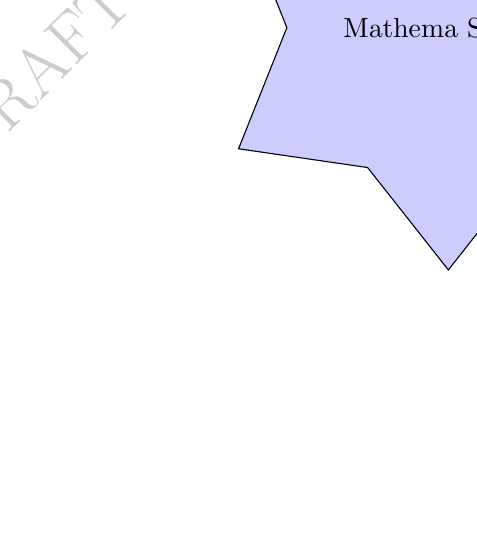
\begin{tikzpicture}
		\tikz \node [fill=blue!20,star,star points=6,draw] {Mathema Shukur };
	\end{tikzpicture}
	\\
	যাদের জন্যে প্রযোজ্যঃ  	\textcolor{magenta}{একাদশ ও দ্বাদশ শ্রেণীর শিক্ষার্থী} \\
	বিষয়ঃ \textcolor{magenta}{উচ্চতর গণিত ১ম পত্র} \\
	অধ্যায়ঃ \textcolor{magenta}{৩-সরলরেখা}\\ 
	Subtopicঃ  \textcolor{magenta}{  দুইটি সরলরেখা পরস্পর সমান্তরাল হওয়ার শর্ত   }\\
	\\
	দুইটি সরলরেখা সমান্তরাল হবে যদি রেখাদ্বয়ের অন্তর্গত কোণ  শূন্য $(0\degree)$ হয় \\
	\\ 
	ঢাল খন্ডন আকার সমীকরণ\\
	$y=m_1x+c_1$ এবং $y=m_2x+c_2$ সরলরেখা দুইটি সমান্তরাল হবে যদি রেখাদ্বয়ের অন্তর্গত কোণ  শূন্য $(0\degree)$ হয় \\
	\begin{align*}
			\tan \theta  &= \frac{m_1-m_2}{1+m_1\,\,m_2}\\
			\\
				\tan  0  &= \frac{m_1-m_2}{1+m_1\,\,m_2}\\
				\\
				0 &= \frac{m_1-m_2}{1+m_1\,\,m_2}\\
				\\
				m_1-m_2 &=0\\
				\\
				m_1&=m_2
	\end{align*}
\\
	দুইটি সরলরেখা সমান্তরাল হবে যদি  রেখা দুইটির ঢাল সমান হয় \\
	\\ 
	\\
	\\
	আদর্শ আকার সমীকরণের ক্ষেত্রে \\
	$a_1x+b_1y+c_1=0$  সরলরেখার ঢাল  $m_1=-\frac{a_1}{b_1}$\\
	\\
		$a_2x+b_2y+c_2=0$  সরলরেখার ঢাল  $m_2=-\frac{a_2}{b_2}$\\
		\\
			$a_1x+b_1y+c_1=0$ এবং 	$a_2x+b_2y+c_2=0$  সরলরেখা দুইটি সমান্তরাল হবে যদি রেখা দুইটির ঢাল সমান হয় \\
			\\
			\begin{align*}
				m_1&=m_2\\
				\\
				-\frac{a_1}{b_1}&=-\frac{a_2}{b_2}\\
				\\
					\frac{a_1}{a_2}&=\frac{b_1}{b_2}\\
			\end{align*}
		\\
		\textcolor{blue}{	$y=m_1x+c_1$ এবং $y=m_2x+c_2$ সরলরেখা দুইটি সমান্তরাল হবে যদি $m_1=m_2$ হয় (ঢাল আকার শর্ত) }\\
		\\
		\textcolor{red}{$a_1x+b_1y+c_1=0$ এবং 	$a_2x+b_2y+c_2=0$  সরলরেখা দুইটি সমান্তরাল হবে যদি $\frac{a_1}{a_2}=\frac{b_1}{b_2}$ হয় (সহগ আকার শর্ত) }\\
		\\
	ঢাকা বোর্ড-২০২১\\ 
 $k$ এর মান কত হলে  $kx+3y+1=0$ এবং  $y=3x+5$ রেখাদ্বয় পরস্পর সমান্তরাল হবে । \\ 
\\
$kx+3y+1=0$ সরলরেখার ঢাল  $m_1=-\frac{k}{3}$\\
\\
$y=3x+5$  সরলরেখার ঢাল  $m_2=3$\\
\\
সমান্তরাল হওয়ার ঢাল আকার শর্ত \\ 
\\
\begin{align*}
	m_1&=m_2\\
	\\
	-\frac{k}{3}&=3\\
	\\
	k&=-9
\end{align*}
\\
	\begin{tikzpicture}[transform shape,scale=1]
	\draw [-latex,thick](-5,0) -- (5,0) node[right] {$x$} coordinate(x axis);
	\draw [-latex,thick](0,-5) -- (0,7) node[above] {$y$} coordinate(y axis);
	\fill[black] (0,0) circle (1 mm);
	\node at (0.3,-0.3) {$\textcolor{purple}{O}$};	
	\node at (-2,3) {$\textcolor{blue}{y=3x+5}$};	
	\node at (3.5,4.5) {$\textcolor{green}{-9x+3y+1=0}$};	
	\draw[very thick,green] (-1.5,-5)--(2,5.8);	
	\draw[very thick,blue] (-3,-4)--(1,8);		
\end{tikzpicture}
\\
	সিলেট বোর্ড-২০২১\\
$kx+y+5=0$	ও $2x-3y+1=0$ রেখাদ্বয় পরস্পর সমান্তরাল হলে $k$ এর  মান কত? \\
\begin{multicols}{2}
\begin{align*}
	kx+y+5&=0\\
	\\
	a_1=k,\quad b_1=1,\quad c_1=5
\end{align*}
\\
\begin{align*}
	2x-3y+1&=0\\
	\\
	a_2=2,\quad b_2=-3,\quad c_2=1
\end{align*}
\end{multicols}
সমান্তরাল হওয়ার সহগ আকার শর্ত \\
\begin{align*}
\frac{a_1}{a_2}&=\frac{b_1}{b_2}\\
\\
\frac{k}{2}&=\frac{1}{-3}\\
\\
k&=-\frac{2}{3}
\end{align*}
\\
\\
\begin{tikzpicture}[transform shape,scale=1]
	\draw [-latex,thick](-5,0) -- (12,0) node[right] {$x$} coordinate(x axis);
	\draw [-latex,thick](0,-7) -- (0,5) node[above] {$y$} coordinate(y axis);
	\fill[black] (0,0) circle (1 mm);
	\node at (0.3,-0.3) {$\textcolor{purple}{O}$};	
	\node at (2,3) {$\textcolor{blue}{2x-3y+1=0}$};	
	\node at (6,0.5) {$\textcolor{green}{-2x+3y+15=0}$};	
	\draw[very thick,green] (-3,-7)--(12,3);	
	\draw[very thick,blue] (-5,-3)--(7,5);		
\end{tikzpicture}
\end{document}